\section{The Analysis of Security and Privacy}
\label{sec:analysis}
In this section, we present the analysis that UPPRESSO achieves the required properties of security and privacy.

\subsection{Adversarial Model}
\label{adver-model}
\textcolor{blue}{Based on the threat model and assumptions in Section \ref{sec:UPPRESSO},
    different adversaries are considered as below.
First of all, in the proofs of security,
    malicious RPs collude with malicious users
        to break any of the four security properties of SSO identity tokens for an honest user to visit an honest RP.
Then, in the analysis of privacy against the IdP-based login tracing,
   an honest-but-curious IdP is the only adversary.
Finally,
    in the privacy analysis against the RP-based identity linkage,
    a number of malicious RPs collude to link an honest user's accounts across these RPs.}

We analyzed UPPRESSO %especially confidentiality and integrity,
     based on a Dolev-Yao style model \cite{SPRESSO}.
% which has been used in the formal analysis of SSO protocols such as OAuth 2.0 \cite{FettKS16} and OIDC \cite{FettKS17}.
The model abstracts the entities in a web system,
    such as web servers and browsers,
    as \emph{atomic processes}. %which communicate with each other through events. % such as HTTPS request and response.
It defines \emph{script processes} to formulate client-side scripts.
%The script is dependently invoked by the browser to process the server-defined logic.
  %such as verifying $Certificate_{RP}$.
%
%postmessage events;
%
%atomic process <-> script process, communication.
%
%Other events change self-trigger.
%
UPPRESSO contains atomic processes including:
an IdP process,
    a finite set of web servers for honest RPs, a finite set of honest browsers, and a finite set of attacker processes.
The processes communicate with each other through events such as HTTPS requests and responses.
%We consider all RP and browser processes are honest,
An RP or a browser controlled by adversaries is modeled as an attacker process.
Within a browser,
 an honest IdP script, an honest RP script, and also attacker scripts which are downloaded from attacker processes,
  are invoked.
%Although the scripts coexist in the same browser, they are strictly separated.
Script processes communicate with each other through \verb+postMessage+,
    modelled as transmitted-to-itself events of a browser process.
%To clearly indicate the action of postMessage communication, we define it as the transmitting-to-itself event of the browser (which is not defined in SPRESSO).

%It contains two honest script processes,
%        downloaded from the RP process and the IdP process, respectively.
% and {\sf script\_attacker} denotes a script downloaded by an attacker process that exists in all browser processes.
%attacker script processes


\textcolor{blue}{After formulating the system by this model,
    we analyze the following data for the proofs in Sections \ref{analysis-security} and \ref{sec-:analysis},
     when there are corresponding adversaries.
We (\emph{a}) trace the lifecycle of an identity token for an honest user to visit an honest RP,
        starting when it is generated and ending when accepted by the RP,
    to ensure it is not leaked to adversaries,
(\emph{b}) 
    locate all places
        where $PID_U$, $PID_{RP}$ and other parameters enclosed in the token are processed,
     to ensure no adversary able to manipulate them,
and (\emph{c})
    locate the places where $PK$ is transmitted and used in the IdP script,
        to ensure no adversary tampering with it.
These conclusions are necessary to prove security of the UPPRESSO protocols.
%
% to ensure it is not leaked to attackers or tampered with by any adversary without checking.
Then,
        we ensure $t$ is unaccessible to the honest-but-curious IdP,
 which is necessary for privacy against the IdP-based login tracing.}

%\emph{Confidentiality} and \emph{integrity} of SSO tokens  in the communications among processes are proved,
%as we locate the generation of a token, and trace all places
%    where $PID_U$, $PID_{RP}$ and other parameters in the token are generated and transmitted,
%     to ensure no adversary able to retrieve or manipulate them.

%The details on the Dolev-Yao web model and the detailed security proofs of UPPRESSO are in the appendix.

%Finally,
%    we formally prove that,
%\emph{user identification}, \emph{RP designation}, \emph{confidentiality}, and \emph{integrity} are fulfilled in UPPRESSO.


\subsection{Security}
\label{analysis-security}
UPPRESSO satisfies four security requirements of SSO identity tokens \cite{ArmandoCCCT08,FettKS16, FettKS17},
     as listed in Section \ref{subsec:basicrequirements}.
%\begin{itemize}
%\setlength{\topsep}{0pt}
%\setlength{\partopsep}{0pt}
%\setlength{\itemsep}{0pt}
%\setlength{\parsep}{0pt}
%\setlength{\parskip}{0pt}
%\item  \textbf{RP Designation}~~
%\item \textbf{User Identification}~~
%\item \textbf{Integrity}~~
%           % and any forged or modified identity token will be rejected.
%\item \textbf{Confidentiality}~~
%\end{itemize}

\vspace{1mm}
\noindent\textcolor{blue}{\textbf{RP Designation.}~~Provided that $r$ is known to only the IdP,
the RP pseudo-identity $PID_{RP} = [t]ID_{RP}$ in the identity token
     designates the target RP with $ID_{RP} = [r]G$, and only this RP.}
%That is,
%    $PID_{RP}$ bound in an identity token is equal to $PID_{RP}$ expected by the target RP;
% and $PID_{RP}$ expected by an RP with $ID_{RP}$,
%    cannot be expected by another RP.

\vspace{0.75mm}
\noindent\textbf{Proof.}
$PID_{RP} = [t]ID_{RP}$ in the the identity token is expected by the target RP,
    because $t$ is also sent to this RP with $ID_{RP}$
     and this RP checks that $PID_{RP}$ is equal to $[t]ID_{RP}$.


Based on the ECDLP
    we prove that,
    for adversaries,
        the probability of finding $t$ and $t'$
    satisfying $[t]ID_{RP_j} = [t']ID_{RP_{j'}}$ is negligible,
    where $RP_j$ and $RP_{j'}$ are any two RPs in the finite set of RPs (i.e.,
    $ID_{RP_j} = [r_j]G$ and $ID_{RP_{j'}} = [r_{j'}]G$, while $r_j$ and $r_{j'}$ are kept secret to adversaries).
This negligible probability means $PID_{RP_j} = [t]ID_{RP_j}$ designates \emph{only} the target RP with $ID_{RP_j}$.

Let $\mathbb{E}$ be an elliptic curve, %over a finite field $\mathbb{F}_q$,
    $G$ be a point on $\mathbb{E}$ of order $n$,
        and $Q = [x]G$ where $x$ is a random integer in $\mathbb{Z}_n$.
Given $G$ and $Q$,
    the probability that a probabilistic polynomial time (PPT) algorithm calculates $x$ (i.e., solves the ECDLP) is negligible.
For any PPT algorithm $\mathcal{D}$ to calculate $x$, we define
\begin{equation*}
{\rm Pr}\{\mathcal{D}(G, [x]G)=x\} = \epsilon_{c}(k)
\end{equation*}
Here, ${\rm Pr}\{\}$ denotes the probability.
So $\epsilon_{c}(k)$ becomes negligible with the increasing security parameter $k$.

Assume a game $\mathcal{G}_c$ between an adversary and a challenger,
    to describe this $PID_{RP}$-collision attack:
the adversary receives a finite set of RP identities from the challenger,
 denoted as ($ID_{RP_1}$, $ID_{RP_2}$, ..., $ID_{RP_m}$)
 where $m$ is the amount of all RPs in the system,
  and then outputs $(a, b, t, t')$.
If $[t]ID_{RP_a}=[t']ID_{RP_b}$, the adversary succeeds in this game.
%If the adversary has the non-negligible probability on succeeding in this game, RP designation is broken.
Note that $m$ is a finite integer, and $m \ll 2^k$ as $k$ increases.
We define the probability that the adversary succeeds in this game as ${\rm Pr}_s$.


\begin{figure}[tb]
  \centering
  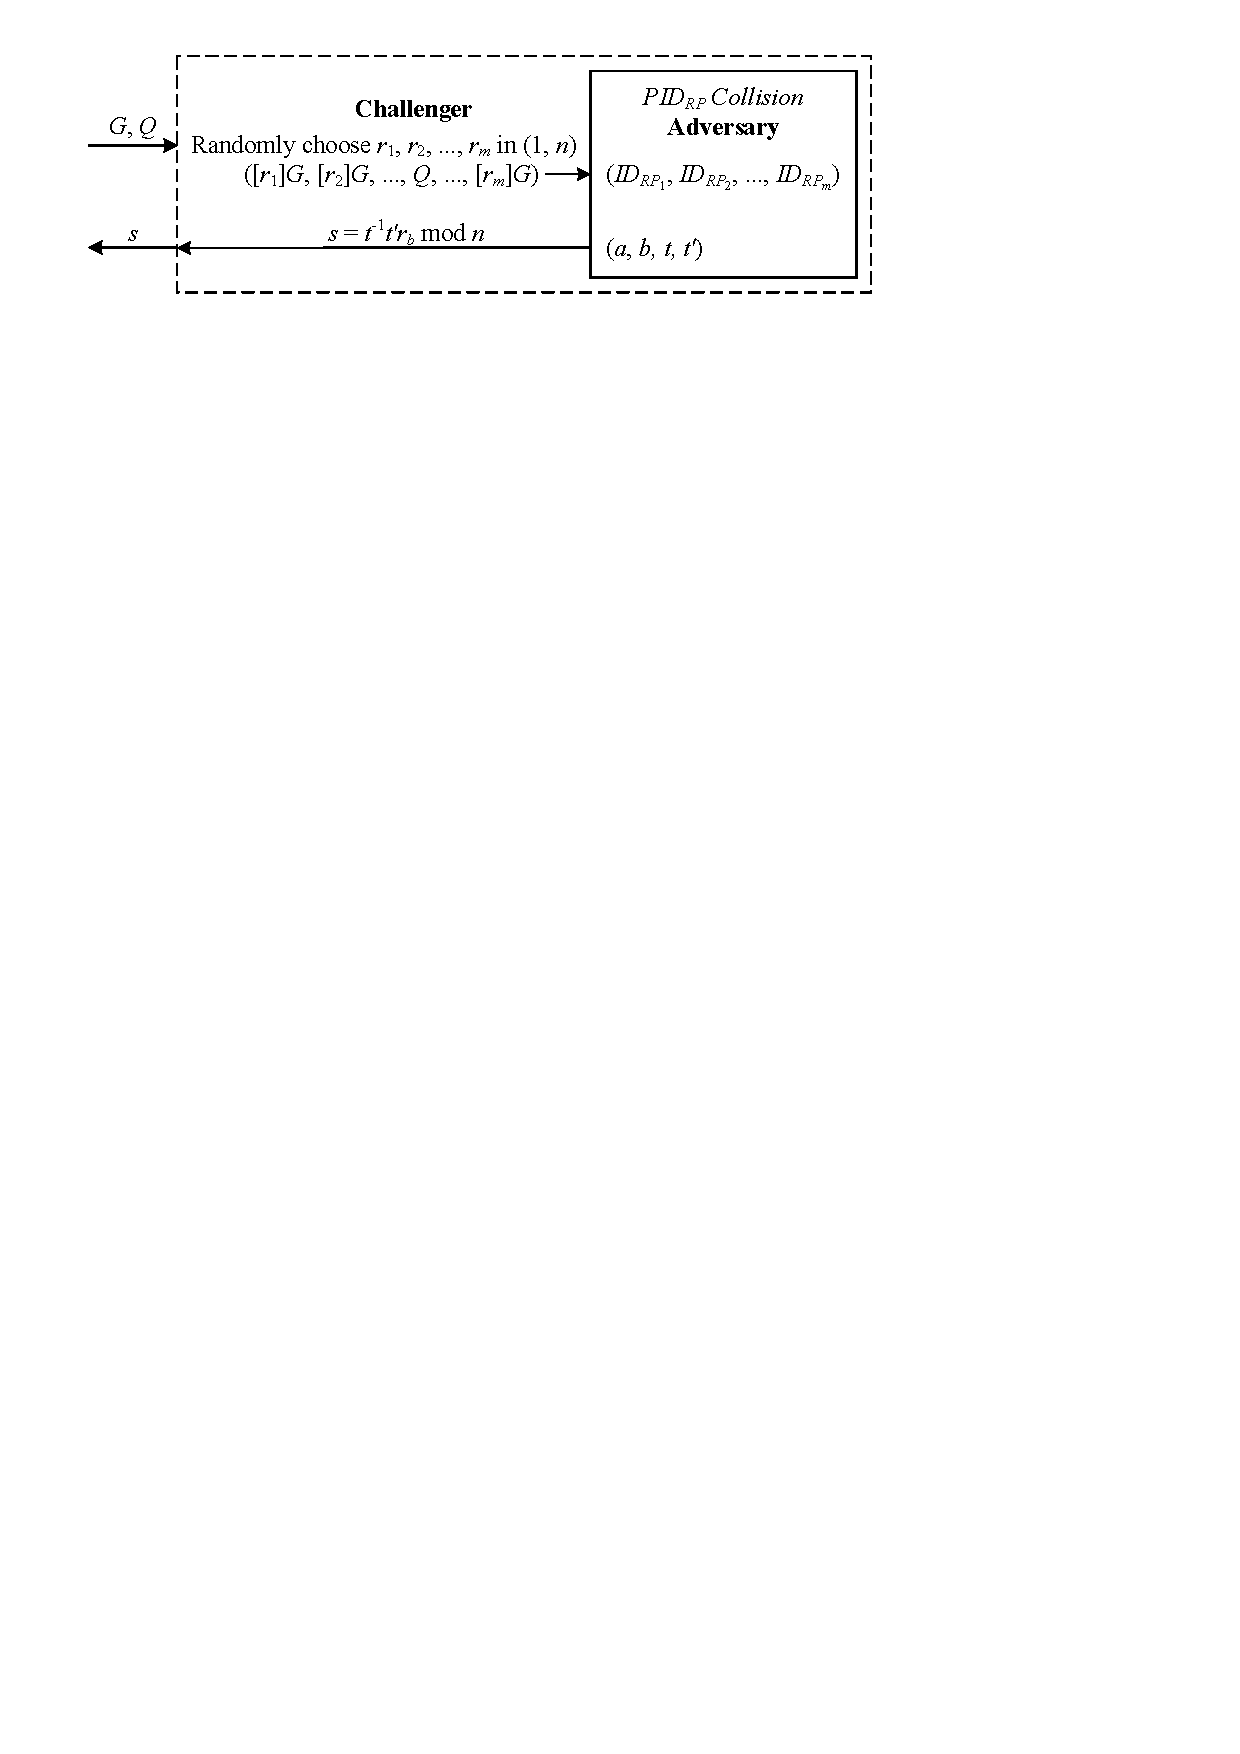
\includegraphics[width=0.97\linewidth]{fig/ecdlp_algorithm.pdf}
  \caption{The algorithm based on the $PID_{RP}$ collision, to solve the ECDLP}
  \label{fig:ecdlp_algorithm}
\end{figure}


Figure \ref{fig:ecdlp_algorithm} shows a PPT algorithm $\mathcal{D}^*_c$ based on this game, to solve the ECDLP.
The input of $\mathcal{D}^*_c$ is in the form of ($G$, $Q$).
On receiving an input, the challenger of $\mathcal{G}_c$ randomly chooses $r_1, r_2, \cdots, r_m$ in $\mathbb{Z}_n$,
 calculates $[r_1]G, [r_2]G, \cdots, [r_m]G$,
 and randomly replaces some $[r_j]G$ with $Q$.
Then,
    these $m$ RP identities are sent to the adversary,
which returns the result ($a$, $b$, $t$, $t'$).
Finally, the challenger of $\mathcal{G}_c$ calculates $s = t^{-1}t'r_b \bmod n$ and returns $s$ as the output of $\mathcal{D}^*_c$.

If $[r_a]G$ happens to be replaced with $Q$ and the adversary of $\mathcal{G}_c$ succeeds,
    we find $Q = [s]G$ and then $s=x$ because $[tr_a]G = [t]Q = [t'r_b]G$.
As $[r_j]G$ is randomly replaced by the challenger,
    $Q$ and other RP identities in the input set are indistinguishable to the adversary.
Thus,
\begin{equation*}
{\rm Pr}\{\mathcal{D}^*_c(G, [x]G)=x\} = {\rm Pr}\{s = x\}={\rm Pr}\{a=j\}{\rm Pr}_s=\frac{1}{m}{\rm Pr}_s
\end{equation*}

If the adversary is able to find $t$ and $t'$
    satisfying that $[t]ID_{RP_j} = [t']ID_{RP_{j'}}$,
    it will have advantages in $\mathcal{G}_c$
        and then
         ${\rm Pr}_s$ becomes non-negligible as $k$ increases.
Because $m$ is a finite integer, ${\rm Pr}\{\mathcal{D}^*_c(G, [x]G)=x\} = \frac{1}{m}{\rm Pr}_s$ also
becomes non-negligible with the increasing $k$.
This violates the ECDLP assumption.
Thus, the probability of finding $t$ and $t'$ satisfying that $[t]ID_{RP_j} = [t']ID_{RP_{j'}}$ in UPPRESSO is negligible,
    so this token binding $PID_{RP}$
     is expected by only the target RP.
$\square$

%If ${\rm Pr}_s$ is non-negligible with the security parameter $k$, ${\rm Pr}\{\mathcal{D}^*_c(G, [x]G)=x\} =\frac{1}{m}{\rm Pr}_s$ is also non-negligible because $m << 2^k$,
%which means that $\mathcal{D}^*_c$ solves the ECDLP.
%So the adversary does not have non-negligible advantages in $\mathcal{G}_c$,
%    and the probability of finding $t$ and $t'$
%    satisfying that $[t]ID_{RP_j} = [t']ID_{RP_{j'}}$ in UPPRESSO is negligible.


%An identity token binding $PID_U$ and $PID_{RP}$,
%    designates the target RP, and only the target RP.
%An honest RP calculates $PID_{RP}$ by itself with the trapdoor $t$ sent from the user,
%    and checks $PID_{RP}$ in the $PID_{RP}$-registration result and the identity token.
%So the target RP will accept this token.

%Meanwhile,
%        the honest IdP guarantees that, within its validity period, the $PID_{RP}$ will be registered only once.
% $PID_{RP}$ will be bound in some identity token.
%An honest RP is ready to accept an identity token binding $PID_{RP}$, only after it receives the signed $PID_{RP}$-registration result.
%Because (\emph{a}) both $PID_{RP}$ and $H(t)$ in the registration result are checked by the RP and then (\emph{b}) the registration result $[PID_{RP}, H(t), Validity]_{SK}$ is acceptable to only one honest RP,
%            the identity token designates only one RP.

\vspace{1mm}
\noindent\textcolor{blue}{\textbf{User Identification.}~~In the identity token
    binding $PID_U$ and $PID_{RP}$,
the user pseudo-identity $PID_U = [ID_U]PID_{RP}$ identifies
        the authenticated user with $ID_U$, % as $Acct = [ID_U][ID_{RP}]$,
         and only this user,  at the target RP with $ID_{RP} = [r]G$.}
%That is,
%in UPPRESSO, $Acct$ identifies the mapping $[ID_u][ID_{RP}]$.

\vspace{0.75mm}
\noindent\textbf{Proof.}
$PID_U$ in identity token identifies the authenticated user as $Acct = [ID_U][ID_{RP}]$
    at the RP with $ID_{RP}$ as follows.
$PID_U = [ID_U]PID_{RP}$ is calculated by the IdP based on the user authenticated as $ID_U = u$, 
    which is analyzed in the Dolev-Yao style model.
In the meantime, the  RP checks that $PID_{RP} = [t]ID_{RP}$
    and calculates $Acct = [t^{-1}]PID_U = [t^{-1}][ID_U]PID_{RP} = [t^{-1}][ID_U][t]ID_{RP} = [ID_U]ID_{RP}$.
%$t$ and $PID_{RP}$ have been checked by the honest RP in the $PID_{RP}$-registration result,
Thus, given a user with $ID_U$, an RP with $ID_{RP}$ always derives an identical account
 $[ID_U]ID_{RP}$ from different identity tokens. % binding $PID_U$ and $PID_{RP}$.
%because in the user's any $i$-th and $i'$-th ($i \neq i'$) login instances to the RP,
% $\mathcal{F}_{Acct}(PID_{U}^i, PID_{RP}^i) = \mathcal{F}_{Acct}(PID_{U}^{i'}, PID_{RP}^{i'}) = [ID_U]ID_{RP}$.

$Acct =  [ID_U]ID_{RP}$ identifies \emph{only} this user.
$\mathbb{E}$ is a finite cyclic group,
    and then $ID_{RP} = [r]G$ is also a generator of order $n$.
Thus, given any RP,
    $[u]ID_{RP}$ assigns a \emph{unique} account to the user,
        provided that $1 \leq u < n$ and $ID_U = u$ is unique. $\square$

%Moreover, adversary may try to provide the
%However, according to the proof of RP designation, there would not be the generated $t$ and $t'$ happening to satisfy that $PID_{RP} = [t]ID_{RP_j} = [tr]G = [t'r']G = [t']ID_{RP_{j'}}$.


%Two malicious users, whose identities are $ID_U = u$ and $ID_{U'} = u'$,
%    could attempt to login to $RP_j$ and $RP_{j'}$, respectively.
%If the generated $t$ and $t'$ happen to satisfy that $PID_{RP} = [t]ID_{RP_j} = [tr]G = [t'r']G = [t']ID_{RP_{j'}}$,
%    these colluding users could arbitrarily choose to register either $[PID_{RP}, PEnpt_U, H(t)]$ or $[PID_{RP}, PEnpt_{U'}, H(t')]$ at the IdP,
%        to receive an identity token binding $PID_{RP}$ and either $PID_U = [u]PID_{RP}$ or $PID_{U'} = [u']PID_{RP}$.\footnote{Such a token designates either $RP_j$ or $RP_{j'}$,
%    but only one honest RP because there is only one acceptable $PID_{RP}$-registration result which is signed by the IdP.
%    So RP designation is not violated in this attack case.}
%When such a token is signed for $RP_j$, the calculated $Acct$ is $[ur]G$ or $[u'r't't^{-1}]G = [u'r]G$;
%    or, when it is signed for $RP_{j'}$, $[urtt'^{-1}]G = [ur']G$ or $[u'r']G$ is calculated.
%That is,
%        even in this collusive case,
%    the calculated account is still the authenticated user's account at the target RP,
%    and it does not result in any attack.


%An adversary might try allure a user to login under the adversary's account,
%    by injecting his identity token into the user's communications with an honest RP.
%Such identity injection attacks are impossible in UPPRESSO as follows.
%If the negotiation of $PID_{RP}$ is not finished yet,
%    the RP will reject the malicious token.
%Even when $PID_{RP}$ has been negotiated,
%    it is kept unknown to the adversary because the communications between two scripts are controlled by a browser
%     and the communications between the browser and the IdP (or the RP) are protected by TLS.
%Thus, an adversary cannot obtain $PID_{RP}$ dynamically negotiated between an honest RP and the user,
%     so it cannot construct an identity token acceptable to the RP.
%

%The detailed process of proof is shown in Appendix.
\vspace{1mm}
\noindent\textcolor{blue}{\textbf{Integrity.}~~An honest RP accepts only identity tokens
 binding its pseudo-identity $PID_{RP}$ and the authenticated user's pseudo-identity $PID_U$,
 and actually binding $ID_{RP}$ and $Acct=[ID_U]ID_{RP}$,
 when $SK$ is held by only the IdP.}

\vspace{0.75mm}
\noindent\textbf{Proof.}
A signed identity token binds $PID_{RP} = [t]ID_{RP}$ and $PID_U = [ID_U]PID_{RP}$,
    % $Acct$ and $ID_{RP}$ implicitly,
    and any breaking results in some failed checking or verification in the login flow as below.
%It is ensured by the IdP's signatures:
First of all, the identity token is signed by the IdP
        and verified by the RP using $PK$,
        so any modification will be rejected.
According to the proof of RP designation,
   % there is no $t' \neq t$ but satisfying that $PID_{RP} = [t]ID_{RP_j} = [t']ID_{RP_{j'}}$.
   $PID_{RP}$ identifies only the RP with $ID_{RP}$;
   according to the proof of user identification,
    $PID_U$ identifiers only the user with $Acct = [ID_U]ID_{RP}$ at the RP.
Therefore, the identity token explicitly binding $PID_U$ and $PID_{RP}$,
    matches \emph{only} one $ID_{RP}$ and \emph{only} one $Acct = [t^{-1}]PID_{U}$.
Thus,
    $Acct$ and $ID_{RP}$ are actually bound in the token by the IdP's signatures,
        due to the one-to-one mapping between (\emph{a}) the pair of $Acct$ and $ID_{RP}$ and (\emph{b}) the triad of $PID_U$, $PID_{RP}$, and $t$. $\square$


%The detailed process of proof is shown in Appendix.

%The detailed process of proof is shown in Appendix.

\vspace{1mm}
\noindent\textcolor{blue}{\textbf{Confidentiality.}~~An identity token
    is accessible to only
                the authenticated user and the target RP, in addition to the IdP signing this token.}

\vspace{0.75mm}
\noindent\textbf{Proof.}
As analyzed in the Dolev-Yao style model, no event leaks an identity token to any malicious entity other than the authenticated user and the designated RP.
First of all, the communications among the IdP, RPs and users,
    are protected by HTTPS,
    and the \verb+postMessage+ HTML5 API ensures the dedicated channels between two scripts within the browser,
    so no other entities can eavesdrop the identity tokens.
Further, the IdP sends an identity token only to the authenticated user
        (i.e., the IdP script).
The IdP script forwards the token to the RP script
 only if it is downloaded from the same origin as $Enpt_{RP}$,
and the binding of $Enpt_{RP}$ and $ID_{RP}$ is ensured by a verified RP certificate.
  %  which is verified by the IdP script.
So only the RP that owns $Enpt_{RP}$ and $ID_{RP}$,
    receives this token. $\square$



\subsection{Privacy}
\label{sec-:analysis}
UPPRESSO effectively prevents the privacy threats of IdP-based login tracing and RP-based identity linkage.

\textcolor{blue}{The information accessible to the IdP and derived from the RP's identity,
    is only $PID_{RP}$ in identity-token requests, where $PID_{RP} = [t]ID_{RP}$ is calculated by a user.
    % and $t$ is kept secret to the IdP.
So the prevention against the IdP-based login tracing in UPPRESSO
    is expressed formally as below.}

\vspace{1mm}
\noindent\textcolor{blue}{\textbf{Privacy against the IdP.}~~If $t$ is random in $\mathbb{Z}_n$ and unknown to the IdP,
the IdP
 cannot infer any information about $ID_{RP}$ or link any pair of $PID_{RP}^i$ and $PID_{RP}^{i'}$
  ($i \neq i'$),
    from an honest user's identity-token requests for $PID_{RP}^i$ ($i = 1, 2, \cdots$).}

\vspace{0.75mm}
\noindent\textbf{Proof.}
Because (\emph{a}) $ID_{RP} = [r]G$ is also a generator of order $n$,
        where $G$ is a generator of finite cyclic group $\mathbb{E}$,
    and (\emph{b}) $t$ is a random number in $\mathbb{Z}_n$ and kept unknown to the IdP,
 from the IdP's view,
 $PID_{RP}$
is \emph{indistinguishable} from a random variable on $\mathbb{E}$.
Thus,
    the IdP cannot infer any information about $ID_{RP}$ from $PID_{RP} = [t]ID_{RP}$,
or distinguish $[t]ID_{RP_j} = [tr]G$ from any other $[t']ID_{RP_{j'}} = [t'r']G$.
So the IdP-based login tracing is impossible. $\square$

\vspace{1mm}
\textcolor{blue}{In every login instance,
    without knowing $u$ and $r$,
    an RP holds $ID_{RP}$ and $Acct$, receives $t$, calculates $PID_{RP}$,
    and verifies $PID_{RP}$ and $PID_U$ in the identity token.
After filtering out the redundant information (i.e., $PID_{RP}= [t]{ID_{RP}}$ and $Acct = [t^{-1}]PID_{U}$),
    the RP actually receives $(ID_{RP}, t, Acct) = ([r]G, t, [ur]G)$.
So the prevention against the RP-based identity linkage in UPPRESSO is expressed as follows.}

\vspace{1mm}
\noindent\textcolor{blue}{\textbf{Privacy against Colluding RPs.}~~Provided that $u$ and $r$ are kept unknown to RPs,
based on the collected information of login instances by $v$ users,
$c$ colluding RPs cannot decide whether a login instance to another RP is initiated by one of these $v$ users or not,
    where
    the collected login instances are denoted as $\mathfrak{L}=\left\{ \begin{matrix}
L_{1,1}, & L_{1,2}, & \cdots, & L_{1,c}\\
L_{2,1}, & L_{2,2}, & \cdots, & L_{2,c}\\
\cdots, & \cdots, & \cdots, & \cdots\\
L_{v,1}, & L_{v,2}, & \cdots, & L_{v,c}
\end{matrix}\right\}$, $L_{i, j} = (ID_{RP_j}, t_{i, j}, [ID_{U_i}]{ID_{RP_j}}) = ([r_j]G, t_{i,j}, [u_ir_j]G)$,
    and the login instance to $RP_{c+1}$ is $L'=(ID_{RP_{c+1}}, t', [ID_{U'}]ID_{RP_{c+1}}) = ([r_{c+1}]G, t', [u'r_{c+1}]G)$.}


\vspace{0.75mm}
\noindent\textbf{Proof.}
We prove this privacy property,
 based on the elliptic curve decisional Diffie-Hellman (ECDDH) assumption. %\cite{GoldwasserK16}.
%That is, while there is the login to an RP, for colluded RPs, they cannot decide whether this login and any logins to other RPs are from the same user.
%
Let $\mathbb{E}$ be an elliptic curve,
    and $G$ be a point on $\mathbb{E}$ of order $n$.
For any PPT algorithm $\mathcal{D}$, the probability of distinguishing
 $([x]G$, $[y]G$, $[xy]G)$ and $([x]G$, $[y]G$, $[z]G)$
is negligible,
 where $x$, $y$ and $z$ are integers randomly and independently chosen in $\mathbb{Z}_n$.
Let  ${\rm Pr}\{\}$ denote the probability and
 we define
\begin{align*}
&{\rm Pr}_1 =  {\rm Pr}\{\mathcal{D}(G, [x]G, [y]G, [xy]G)=1\} \\
&{\rm Pr}_2 =  {\rm Pr}\{\mathcal{D}(G, [x]G, [y]G, [z]G)=1\}
\end{align*}
So $\epsilon_{r}(k) = |{\rm Pr}_1 - {\rm Pr}_2|$ becomes negligible as $k$ increases.

\begin{figure}[tb]
  \centering
  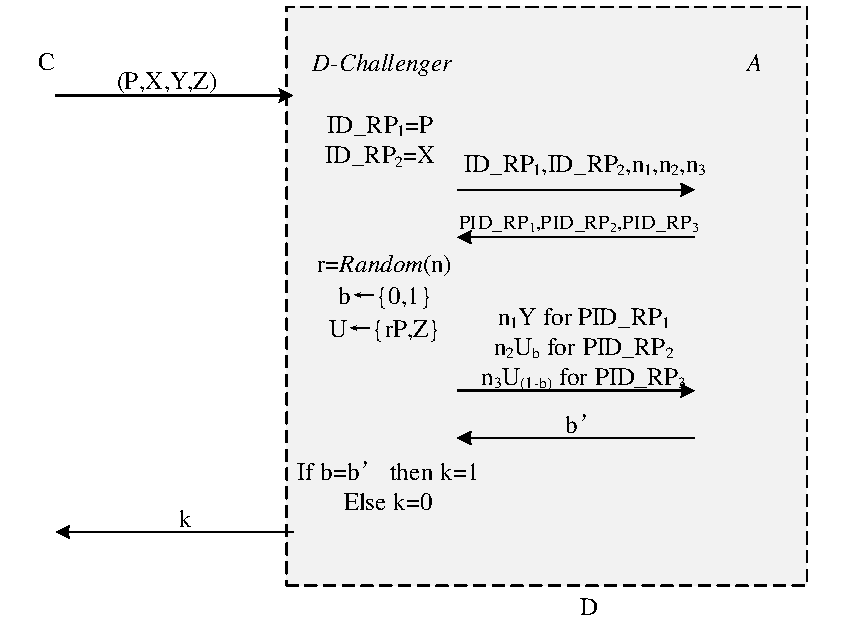
\includegraphics[width=0.97\linewidth]{fig/dalgorithm.pdf}
  \caption{The algorithm based on the RP-based identity linkage, to solve the ECDDH problem}
  \label{fig:dalgorithm}
\end{figure}

We define the RP-based identity linkage game $\mathcal{G}_r$:
after receiving $\mathfrak{L}$ and $L'$ from a challenger,
    the adversary outputs the result $s = 1$ if it decides $u' \in \{u_1, u_2, \cdots, u_v\}$ or $s = 0$ if $u'$ is randomly chosen in $\mathbb{Z}_n$.
The adversary's advantage in $\mathcal{G}_r$ is defined as $\mathbf{Adv}_{A}$.
%If the adversary is able to distinguish whether $u' \in \{u_1, u_2, \cdots, u_v\}$ or not,
%    the adversary will have non-negligible advantages in $\mathcal{G}_r$
%        and ${\rm Adv}_A$ is non-negligible.
Then,
\begin{align*}
&{\rm Pr}'_1={\rm Pr}\{\mathcal{G}_r(\mathfrak{L}, L'|ID_{U'} \in \{ID_{U_1}, ID_{U_2}, \cdots, ID_{U_v}\})=1\} \\
&{\rm Pr}'_2={\rm Pr}\{\mathcal{G}_r(\mathfrak{L}, L'|ID_{U'} \in \mathbb{Z}_n)=1\}\\
&{\mathbf{Adv}}_{A}=|{\rm Pr}'_1-{\rm Pr}'_2|
\end{align*}

We design a PPT algorithm $\mathcal{D}^*_r$ based on $\mathcal{G}_r$, shown in Figure \ref{fig:dalgorithm}, to solve the ECDDH problem.
The input is in the form of $(G$, $Q_1=[x]G$, $Q_2=[y]G$, $Q_3=[z]G)$.
On receiving the input, the challenger of $\mathcal{G}_r$ randomly chooses
 $\{u_1, u_2, \cdots, u_v\}$, $\{r_1, r_2, \cdots, r_c\}$, $\{t_{1, 1}, t_{1, 2}, \cdots, t_{v, c}\}$, and $t'$ in $\mathbb{Z}_n$.
Then the challenger constructs $\mathfrak{L}$ and $L'$ as below.
It firstly assigns $L_{i, j} = ([r_j]G, t_{i, j}, [u_ir_j]G)$, %$1\leq i \leq v$ and $1\leq j \leq c$,
    and randomly chooses $d \in [1, v]$ to
 replace $[u_d r_j]G$ with $[r_j]Q_1=[xr_j]G$ for $1\leq j \leq c$.
So $\mathfrak{L}=\left \{ \begin{matrix}
L_{1,1},&L_{1,2},&\cdots,&L_{1,c}\\
L_{2,1},& L_{2,2},&\cdots,&L_{2,c}\\
\cdots,&\cdots,&\cdots,&\cdots\\
([r_{1}]G, t_{d, 1}, [r_{1}]Q_1),&\cdots,&\cdots,&([r_{c}]G, t_{d, c}, [r_{c}]Q_1)\\
\cdots,&\cdots,&\cdots,&\cdots\\
L_{v,1},&L_{v,2},&\cdots,&L_{v,c}
\end{matrix}\right\}$.
%$L=$\{($[r_1]G$, $t_{1, 1}$, $[[u_1][r_1]G$), ($[r_2]G$, $t_{1, 2}$, $[u_1][r_2]G$), $\cdots$, ($[r_{\beta}]G$, $t_{\alpha, \beta}$, $[r_{\beta}]Q_1$), $\cdots$, ($[r_b]G$, $t_{a, b}$, $[u_a][r_b]G$)\}
%
The challenger assigns $L' = (Q_2, t', Q_3) = ([y]G, t', [z/y][y]G)$.
Finally,
    $\mathfrak{L}$ and $L'$ are sent to the adversary,
        and the output $s$ of $\mathcal{G}_r$ is output by the challenger.
According to the above construction of $\mathfrak{L}$ and $L'$,
    $x$ is actually inserted into $\mathfrak{L}$ as $u_d$
    and $z/y$ is assigned to $u'$.
So, if $z = xy$, then $z/y=x$ and $ID_{U'} \in \{ID_{U_1}, ID_{U_2}, \cdots, ID_{U_v}\}$;
    otherwise, $ID_{U'} \in \mathbb{Z}_n$.
Thus,
\begin{align*}
&{\rm Pr}_1={\rm Pr}\{\mathcal{D}^*_r(G, [x]G, [y]G, [xy]G)=1\}={\rm Pr}'_1 \\=&  {\rm Pr}\{\mathcal{G}_r(\mathfrak{L}, L'|ID_{U'} \in \{ID_{U_1}, ID_{U_2}, \cdots, ID_{U_v}\})=1\} \\
&{\rm Pr}_2={\rm Pr}\{\mathcal{D}^*_r(G, [x]G, [y]G, [z]G)=1\} ={\rm Pr}'_2 \\=&  {\rm Pr}\{\mathcal{G}_r(\mathfrak{L}, L'|ID_{U'} \in \mathbb{Z}_n)=1\}\\
&{\mathbf{Adv}}_{A}=|{\rm Pr}'_1-{\rm Pr}'_2|=|{\rm Pr}_1-{\rm Pr}_2|=\epsilon_{r}(k)
\end{align*}

The ECDDH assumption means that in $\mathcal{G}_r$ the adversary does not have advantages,
    i.e., cannot distinguish a user $U'$ chosen from \{${U_1}, {U_2}, \cdots, {U_v}$\}
        or randomly from the universal user set.
%    (indistinguishability of users to colluding RPs).
So the RP-based identity linkage is impossible. $\square$


%    the adversary will have non-negligible advantages in $\mathcal{G}$
%        and $Pr_s$ is non-negligible.

%If $s'=1$ and $ID_U' \in$\{$ID_{U_1}$, $ID_{U_2}$, ..., $ID_{U_a}$\}, the adversary succeeds in this game.
%If the adversary does not have the non-negligible probability on succeeding in this game, RP-based identity linkage is not impossible.

%We define the probability that the adversary succeeds in this game as $Pr_s'$.
%So, if the adversary is able to ,
%    the adversary will have non-negligible advantages in $\mathcal{G}$
%        and $Pr_s$ is non-negligible.
